\documentclass[
12pt,
spanish,
singlespacing,
parskip,
headsepline,]{article}
\usepackage{inputenc}
\usepackage[spanish]{babel}
\usepackage{palatino}
\usepackage{graphicx}
\usepackage{float}
\renewcommand{\labelenumii}{\theenumii}
\renewcommand{\theenumii}{\theenumi.\arabic{enumii}.}

%opening
\title{Monitoreo y control de radares ATSA}
\author{Gonzalo Nahuel Vaca}

\begin{document}

\maketitle
\thispagestyle{empty}

\begin{abstract}

Este documento es una propuesta de proyecto en el marco de la Maestría en Internet de las Cosas de la Universidad de Buenos Aires.

\end{abstract}

\newpage

\tableofcontents

\newpage

\section{Propósito del proyecto}

La Universidad de Buenos Aires (UBA) solicita que sus candidatos de Maestría realicen un proyecto que consuma 600 horas de ingeniería.
Las características técnicas esperadas son las siguientes:

\begin{itemize}
	\item Percepción: programación y diseño de dispositivos embebidos.
	\item Transporte: uso de protocolos de comunicación.
	\item Procesamiento: persistencia y análisis de datos.
	\item Aplicación: interfaz gráfica de usuario.
	\item Negocio: gestión y monitoreo del sistema.
\end{itemize}

Las dificultades que enfrenta el sistema de radares se pueden solucionar con un proyecto que cumpla los requerimientos de UBA.
A continuación se enumeran los problemas identificados:

\begin{itemize}
	\item Persistencia: la arquitectura de datos no es adecuada para el volumen de información manejado, no es escalable y no es posible ofrecer un servicio profesional de análisis de datos.
	\item Comunicación con radares: los puntos de agregación funcionan con aplicaciones antiguas que no están correctamente integradas al sistema operativo.
	\item Interfaz gráfica: su aspecto es antiguo, no es apta para \emph{smartphones} y su funcionalidad es lenta y limitada.
	\item \emph{Software} sin licencias: la solución actual carece de soporte en puntos críticos y aumenta la superficie de posibles fallas.
\end{itemize}

\section{Descripción técnica-conceptual del proyecto a realizar}

La compañía ATSA debe cumplir con los requerimientos de servicios demandados por los clientes.
En particular, ofrecer un sistema de telemetría para monitorear y controlar los radares vehiculares.
Además se debe acceder a los datos históricos de los dispositivos.

El proyecto constará de un \emph{datalogger} ATSA que estará conformado por una plataforma embebida.
Esta plataforma cumplirá la función de punto de agregación con los dispositivos en campo y se comunicará con un \emph{modem GSM} para acceder a la Internet.
Además deberá presentar una interfaz gráfica que permita verificar su funcionamiento, modificar su configuración y acceder a los datos que se encuentren guardados dentro del \emph{datalogger} ATSA.
Finalmente, el equipo deberá utilizar un protocolo de comunicación confiable que minimice el uso de datos.

El cliente tendrá a su disposición una interfaz gráfica que le permita acceder a un sistema ATSA.
Esta solución permitirá ver todos los datos históricos de sus dispositivos, como así también, las novedades de funcionamiento de sus equipos.
Además, se le ofrecerá una \emph{API} que permita conectar un sistema propio con el de ATSA.

Se creará una interfaz gráfica para los operadores de ATSA.
Esto permitirá vender suscripciones del tipo \emph{Helpdesk}.
Además, se podrá ofrecer al cliente un producto adicional que permita transferir todo el monitoreo y control a los operadores de ATSA.

El proyecto deberá cumplir con los actuales estándares de ciberseguridad y protección de la propiedad intelectual de ATSA.
Con la finalidad de proteger el patrimonio y reputación de la compañía.

Se construirá una arquitectura de datos que pueda manejar el volumen de información demandado. Esta base de datos permitirá usar el sistema \emph{legacy} y un posible futuro sistema de aprendizaje automático.

En el diagrama presente en la figura \ref{fig:general} se puede observar un esquema del proyecto a realizar y su interacción con las distintas entidades.

\begin{figure}[h!]
	\centering
	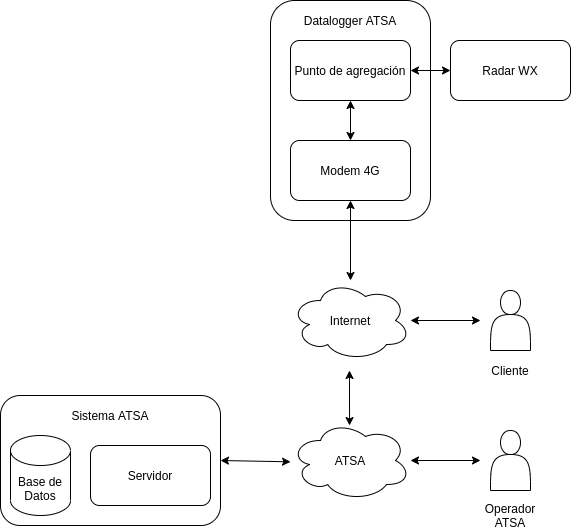
\includegraphics[width=\textwidth]{Figuras/diagramaGeneral.png}
	\caption{diagrama general del proyecto.}
	\label{fig:general}
\end{figure}

\section{Alcance del proyecto}

El proyecto incluye en su alcance la creación de un servicio embebido que recoja la información de los radares \emph{Exemis}.
Ofrecerá conexión \emph{GSM} para realizar acceder a la Internet.
Además, se deberá resolver la comunicación con un servidor que forma parte del desarrollo.
El servidor ofrecerá una interfaz de programación de aplicaciones (API) que permitirá el monitoreo y control de los radares.

Se creará una arquitectura de persistencia moderna que permita la gestión de grandes volúmenes de datos.
Deberá ofrecer posibilidad de implementar futuros estudios de aprendizaje automático.
Además, el sistema deberá ser compatible con el \emph{legacy}.
Finalmente, los datos serán georreferenciados para soportar radares móviles y consultas geográficas.

Se desarrollará una interfaz gráfica de usuario que siga un patrón de diseño \emph{material design} y se comportará adecuadamente según el tamaño de la pantalla del dispositivo utilizado.


\section{Supuestos del proyecto}

Para el desarrollo del presente proyecto se supone que se tendrá acceso a la documentación necesaria para implementar una comunicación con los radares Exemys.
Además se espera tener acceso al sistema actual con la finalidad de portarlo como \emph{legacy}.

Se espera tener una copia del manual de marca de ATSA con el fin de utilizar la paleta de colores, la tipografía y las reglas de diseño gráfico de la compañía. Se supone que se tendrá una copia de los archivos de tipografía e iconografía.

Finalmente se necesita tener acceso a la red de ATSA para realizar las pruebas que se consideren necesarias. Además de disponer de una infraestructura de desarrollo \emph{GitLab}.

\section{Requerimientos}

\begin{enumerate}
	\item Grupo de requerimientos asociados al \emph{datalogger} ATSA
		\begin{enumerate}
			\item Debe implementar el protocolo del radar
			\item Debe leer las mediciones del radar
			\item Debe persistir las mediciones del radar
			\item Debe leer el estado del radar
			\item Debe persistir estados anormales del radar
			\item Debe comunicarse con el sistema ATSA
			\item Debe presentar una interfaz gráfica de monitoreo y control
		\end{enumerate}	
	\item Grupo de requerimientos asociados al servidor del sistema ATSA
		\begin{enumerate}
			\item Debe autentificar a los usuarios
			\item Debe autentificar a los dispositivos
			\item Debe autentificar a los operadores
			\item Debe comunicarse con la base de datos
			\item Debe permitir realizar consultas a la base de datos y descargar los resultados
			\item Las comunicaciones con entidades externas deberán ser cifradas
			\item Debe ser compatible con el sistema \emph{legacy}
			\item Debe ser compatible con soluciones \emph{cloud}
		\end{enumerate}
	\item Grupo de requerimientos asociados a la base de datos del sistema ATSA
		\begin{enumerate}
			\item Debe manejar grandes volúmenes de datos
			\item Debe manejar datos georreferenciados
			\item Debe manejar consultas georreferenciadas
			\item Debe persistir contraseñas de manera cifrada
			\item Debe ser compatible con soluciones de \emph{data center}
		\end{enumerate}
	\item Grupo de requerimientos asociados a la interfaz de operador ATSA
		\begin{enumerate}
			\item Debe ser ergonómica
			\item Debe permitir ver en vivo el estado de los dispositivos
		\end{enumerate}
	\item Grupo de requerimientos asociados a la interfaz de cliente
		\begin{enumerate}
			\item Debe ser responsiva
			\item Debe tener un aspecto moderno y corporativo
			\item Debe ser ligera para la infraestructura de ATSA
		\end{enumerate}
\end{enumerate}

\section{Entregables principales del proyecto}

\begin{itemize}
	\item Código fuente. 
	\item Documentación técnica interna de ATSA.
	\item Documentación de API para clientes.
	\item Manual de usuario.
	\item Un \emph{datalogger} ATSA funcionando.
	\item Un sistema ATSA funcionando.
\end{itemize}

\section{Desglose del trabajo en tareas}

\begin{enumerate}
	\item \textbf{Planificación (25 hs)}
	\begin{enumerate}
		\item Relevamiento de las necesidades (5 hs)
		\item Análisis de requerimientos (10 hs)
		\item Confección de la planificación del proyecto (10 hs)
	\end{enumerate}
	\item \textbf{Diseño de la base de datos (225 hs)}
	\begin{enumerate}
		\item Elección de tecnología (15 hs)
		\item Diseño de la arquitectura de datos (50 hs)
		\item Diseño de pruebas (20 hs)
		\item Escritura del código (30 hs)
		\item Puesta en marcha (35 hs)
		\item Replicación de los datos \emph{legacy} (40 hs)
		\item Pruebas de funcionamiento (35 hs)
	\end{enumerate}
	\item \textbf{Diseño del servidor ATSA (100 hs)}
	\begin{enumerate}
		\item Elección de tecnología (5 hs)
		\item Diseño de pruebas de base de datos (10 hs)
		\item Escritura de código de conexión con base de datos (15 hs)
		\item Pruebas de comunicación con base de datos (5 hs)
		\item Diseño de pruebas de sesión (5 hs)
		\item Escritura de código del sistema de sesión (10 hs)
		\item Pruebas del sistema de sesión (5 hs)
		\item Diseño de pruebas de comunicación con dispositivos (5 hs)
		\item Escritura de código de comunicación con dispositivos (10 hs)
		\item Pruebas de comunicación con dispositivos (5 hs)
		\item Diseño de pruebas de comunicación en vivo (5 hs)
		\item Escritura de código de comunicación en vivo (15 hs)
		\item Pruebas de comunicación en vivo (5 hs)
	\end{enumerate}
	\item \textbf{Programación de la interfaz de operador ATSA (25 hs)}
	\begin{enumerate}
		\item Selección de \emph{framework} (5 hs)
		\item Escritura de código (10 hs)
		\item Pruebas con humanos (10 hs)
	\end{enumerate}
	\item \textbf{Programación de la interfaz de usuario (25 hs)}
	\begin{enumerate}
		\item Selección de \emph{framework} (5 hs)
		\item Escritura de código (10 hs)
		\item Pruebas con humanos (10 hs)
	\end{enumerate}
	\item \textbf{Diseño del \emph{datalogger} ATSA (200)}
	\begin{enumerate}
		\item Elección de plataforma embebida (20 hs)
		\item Elección de tecnologías de firmware (20 hs)
		\item Diseño de pruebas de funcionamiento (30 hs)
		\item Escritura del firmware (40 hs)
		\item Pruebas de funcionamiento (20 hs)
		\item Diseño de la interfaz gráfica (40 hs)
		\item Pruebas de funcionamiento con humanos (30 hs)
	\end{enumerate}
\end{enumerate}

\textbf{Cantidad total de horas: 600 hs}

\section{Diagrama de Activity On Node}

\begin{figure}[H]
	\centering
	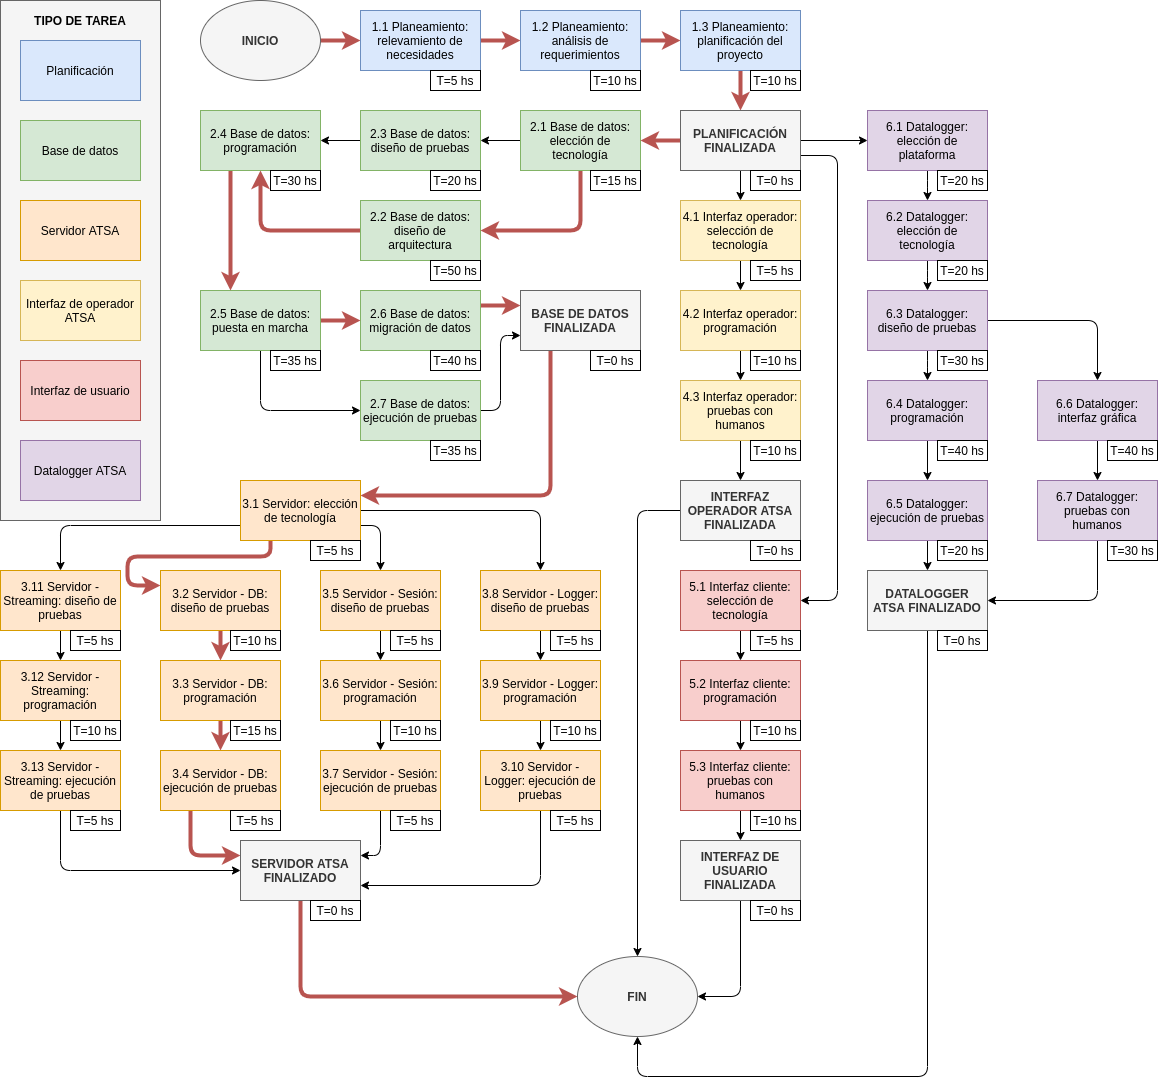
\includegraphics[width=\textwidth]{Figuras/ActivityOnNode.png}
	\caption{diagrama de Activity On Node.}
	\label{fig:activity}
\end{figure}

\section{Diagrama de Gantt}

El diagrama de Gantt fue confeccionado tomando 12 horas de trabajo semanales del responsable del proyecto fuera del horario laboral de ATSA.
Se estiman 12 meses de duración bajo este esquema.
La planificación se puede observar en las figuras \ref{fig:gantt1}, \ref{fig:gantt2}, \ref{fig:gantt3}, \ref{fig:gantt4}, \ref{fig:gantt5}, \ref{fig:gantt6} y \ref{fig:gantt7}.

\begin{figure}[H]
	\centering
	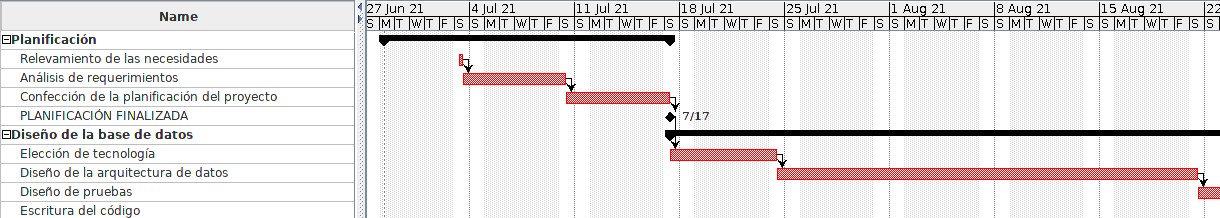
\includegraphics[width=\textwidth]{Figuras/gantt01.png}
	\caption{diagrama de Gantt, parte 1.}
	\label{fig:gantt1}
\end{figure}

\begin{figure}[H]
	\centering
	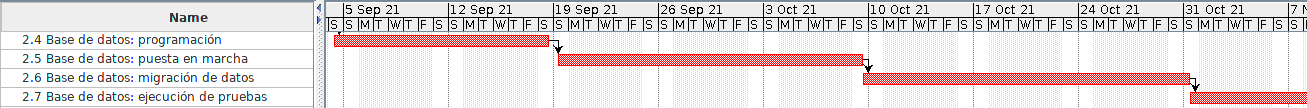
\includegraphics[width=\textwidth]{Figuras/gantt02.png}
	\caption{diagrama de Gantt, parte 2.}
	\label{fig:gantt2}
\end{figure}

\begin{figure}[H]
	\centering
	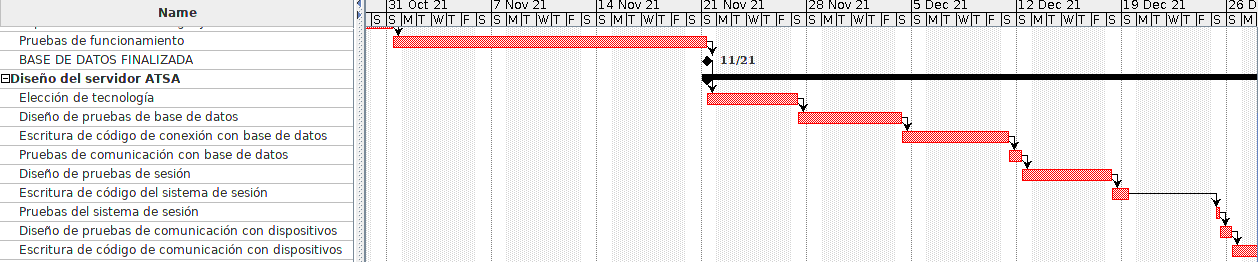
\includegraphics[width=\textwidth]{Figuras/gantt03.png}
	\caption{diagrama de Gantt, parte 3.}
	\label{fig:gantt3}
\end{figure}

\begin{figure}[H]
	\centering
	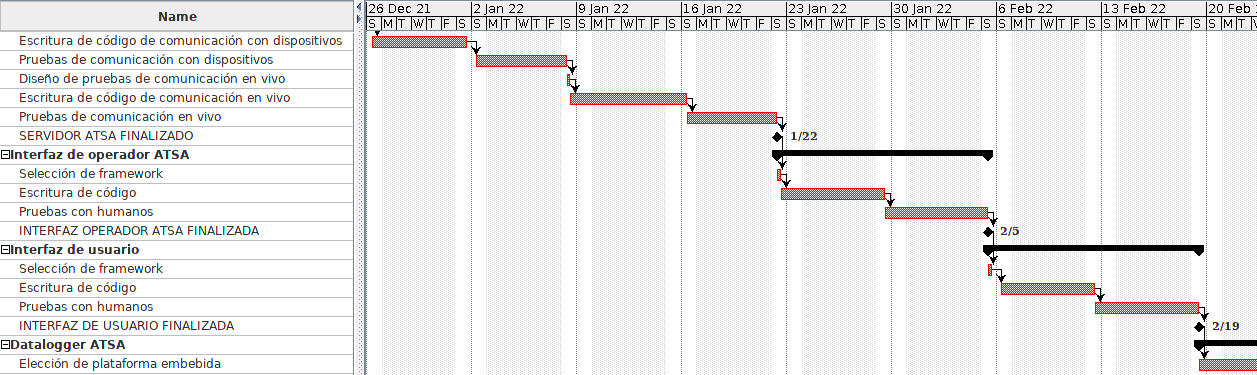
\includegraphics[width=\textwidth]{Figuras/gantt04.png}
	\caption{diagrama de Gantt, parte 4.}
	\label{fig:gantt4}
\end{figure}

\begin{figure}[H]
	\centering
	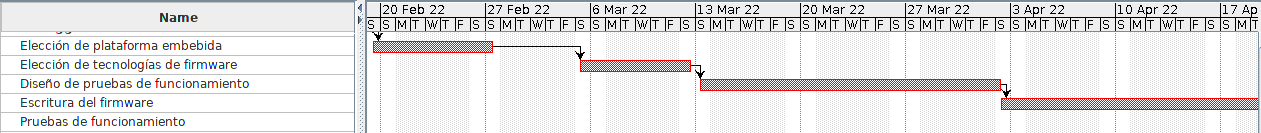
\includegraphics[width=\textwidth]{Figuras/gantt05.png}
	\caption{diagrama de Gantt, parte 5.}
	\label{fig:gantt5}
\end{figure}

\begin{figure}[H]
	\centering
	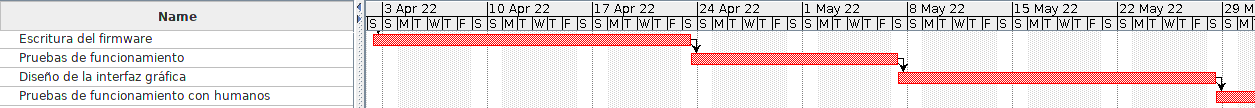
\includegraphics[width=\textwidth]{Figuras/gantt06.png}
	\caption{diagrama de Gantt, parte 6.}
	\label{fig:gantt6}
\end{figure}

\begin{figure}[H]
	\centering
	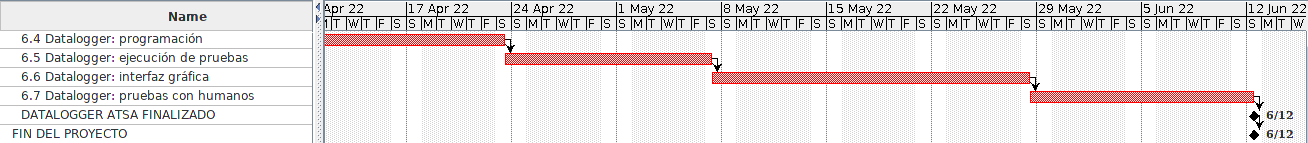
\includegraphics[width=\textwidth]{Figuras/gantt07.png}
	\caption{diagrama de Gantt, parte 7.}
	\label{fig:gantt7}
\end{figure}

\section{Matriz de asignación de responsabilidades}

Las referencias para leer la matriz de asignación de responsabilidades son las siguientes:

\begin{itemize}
	\item P = Responsabilidad primaria
	\item S = Responsabilidad secundaria
	\item A = Aprobación
	\item I = Informado
	\item C = Consultado
\end{itemize}

A continuación se muestran las tablas de asignación de responsabilidades:

\begin{table}[H]
	\centering
	\begin{tabular}{cccc}
		Código WBS & \begin{tabular}[c]{@{}c@{}}Gonzalo Vaca\\ Responsable\end{tabular} & \begin{tabular}[c]{@{}c@{}}Marcelo Macchi\\ Orientador\end{tabular} & \begin{tabular}[c]{@{}c@{}}Daniel Bettatis\\ Cliente\end{tabular} \\ \hline
		1.1 & S & P & I \\
		1.2 & P & C &   \\
		1.3 & P & A & I \\
		2.1 & P & C &   \\
		2.2 & P & I &   \\
		2.3 & P & C &   \\
		2.4 & P & I &   \\
		2.5 & S & P & I \\
		2.6 & P & S & A \\
		2.7 & P & A & I \\
		3.1 & P & C & I \\
		3.2 & P & C &   \\
		3.3 & P & I &   \\
		3.4 & P & A & I \\
		3.5 & P & A &   \\
		3.6 & P & I &   \\
		3.7 & P & A & I \\
		3.8 & P & C &   \\
		3.9 & P & I &   \\
		3.10 & P & A & I \\
		3.11 & P & C &  \\
		3.12 & P & I &  \\
		3.13 & P & A & I
	\end{tabular}
\end{table}

\begin{table}[H]
	\centering
	\begin{tabular}{cccc}
		Código WBS & \begin{tabular}[c]{@{}c@{}}Gonzalo Vaca\\ Responsable\end{tabular} & \begin{tabular}[c]{@{}c@{}}Marcelo Macchi\\ Orientador\end{tabular} & \begin{tabular}[c]{@{}c@{}}Daniel Bettatis\\ Cliente\end{tabular} \\ \hline
		4.1 & P & I &  \\
		4.2 & P & I &  \\
		4.3 & P & A & I \\
		5.1 & P & I &  \\
		5.2 & P & I &  \\
		5.3 & P & A & I \\
		6.1 & P & S & C \\
		6.2 & P & C &  \\
		6.3 & P & I &  \\
		6.4 & P & I &  \\
		6.5 & P & A & I \\
		6.6 & P & C &  \\
		6.7 & P & A & I
	\end{tabular}
\end{table}

\section{Procesos de cierre}

Establecer las pautas de trabajo para realizar una reunión final de evaluación del proyecto, tal que contemple las siguientes actividades:

\begin{itemize}
	\item El responsable del proyecto analizará si se respetó el plan de proyecto original, comparando dicho cronograma contra el real e identificando las tareas que mayor divergencia de tiempo presentaron y sus causas.
	\item El responsable del proyecto realizará una lista de las técnicas y procedimientos que le resultaron útiles para cumplir con los objetivos preestablecidos, y las que le hayan generado retrasos, indicando las posibles causas.
	\item El responsable del proyecto se encargará de agradecer a todas las personas involucradas en el proyecto.
\end{itemize}

\end{document}
